%% This is an example first chapter.  You should put chapter/appendix that you
%% write into a separate file, and add a line \include{yourfilename} to
%% main.tex, where `yourfilename.tex' is the name of the chapter/appendix file.
%% You can process specific files by typing their names in at the 
%% \files=
%% prompt when you run the file main.tex through LaTeX.
\chapter{Use Case 2 - Drug-Side Only Input}

\emph{Use case} ini melibatkan hanya satu sisi yaitu \emph{Drug-side} saja. pada \emph{use case} ini, input dari salah satu \emph{drug-side} (Plant atau Compound) harus ada.

\section{Plant Search Only}

Pada contoh ini, input dari \emph{drug-side} berupa tanaman (Plant). Contoh ini mencari dari tanaman yang diinputkan, apa saja senyawa yang terkandung dalam tanaman itu, dan senyawa tersebut dapat berkhasiat untuk penyakit apa melalui protein apa.

\subsection{Input}
\begin{figure}[H]
	\centering
	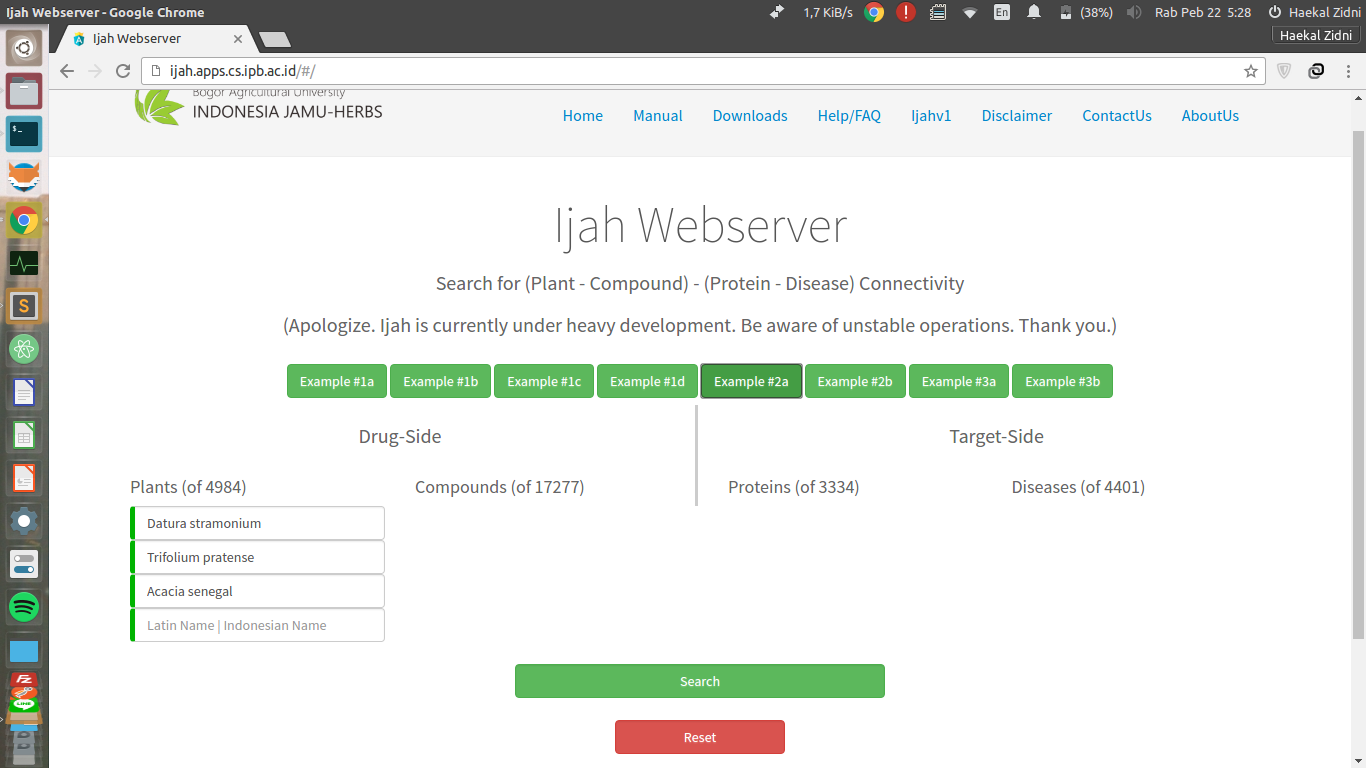
\includegraphics[scale=0.3]{example_2a.png}
	\caption{Contoh \emph{use case} input Plant Search Only}
	\label{fig:example_2a}
\end{figure}

Seperti yang telah dibahas pada bab sebelumnya, untuk jenis \emph{use case} ini tombol hanya bertuliskan \textbf{Search}, bukan Search and Predict seperti \emph{use case} sebelumnya.

\subsection{Output}
Output pada contoh \emph{search} dari 3 jenis tanaman ini adalah sebagai berikut, dimulai dari \emph{Connectivity Graph Output}

\begin{figure}[H]
	\centering
	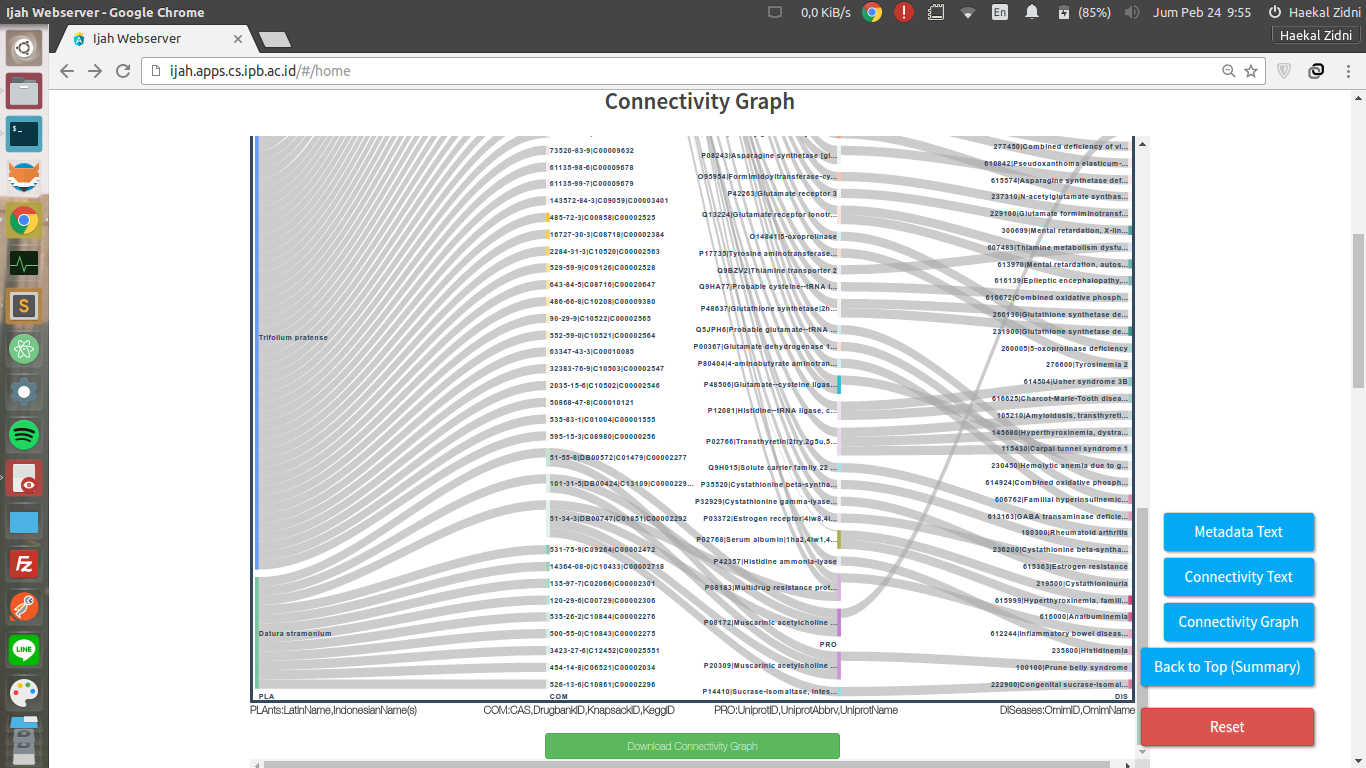
\includegraphics[scale=0.3]{ijah_example_2a_graph.png}
	\caption{Connectivity Graph Output pada use case Plant Search Only}
	\label{fig:ijah_example_2a_output}
\end{figure}

Graf yang dihasilkan kali ini cukup besar karena menampilkan semua penyakit yang terkait dengan seluruh senyawa yang dikandung tanaman-tanaman tersebut. Karena contoh ini menampilkan semua yang terkait dengan tanaman yang diinputkan.

Hasil \emph{Connectivity Text Output} untuk contoh ini:

\begin{figure}[H]
	\centering
	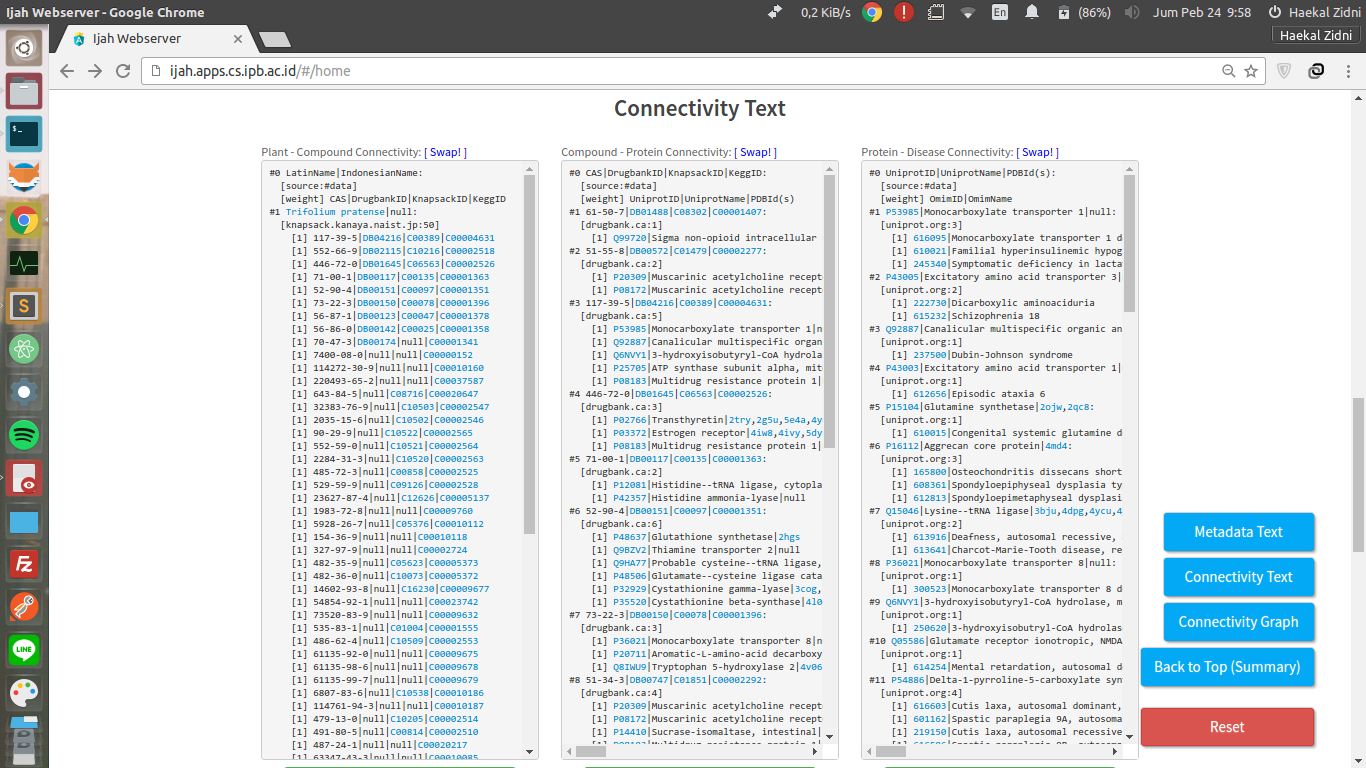
\includegraphics[scale=0.3]{ijah_example_2a_text.png}
	\caption{Connectivity Text Output pada use case Plant Search Only}
	\label{fig:ijah_example_2a_text}
\end{figure}

Hasil \emph{Metadata Text Output} untuk contoh ini:

\begin{figure}[H]
	\centering
	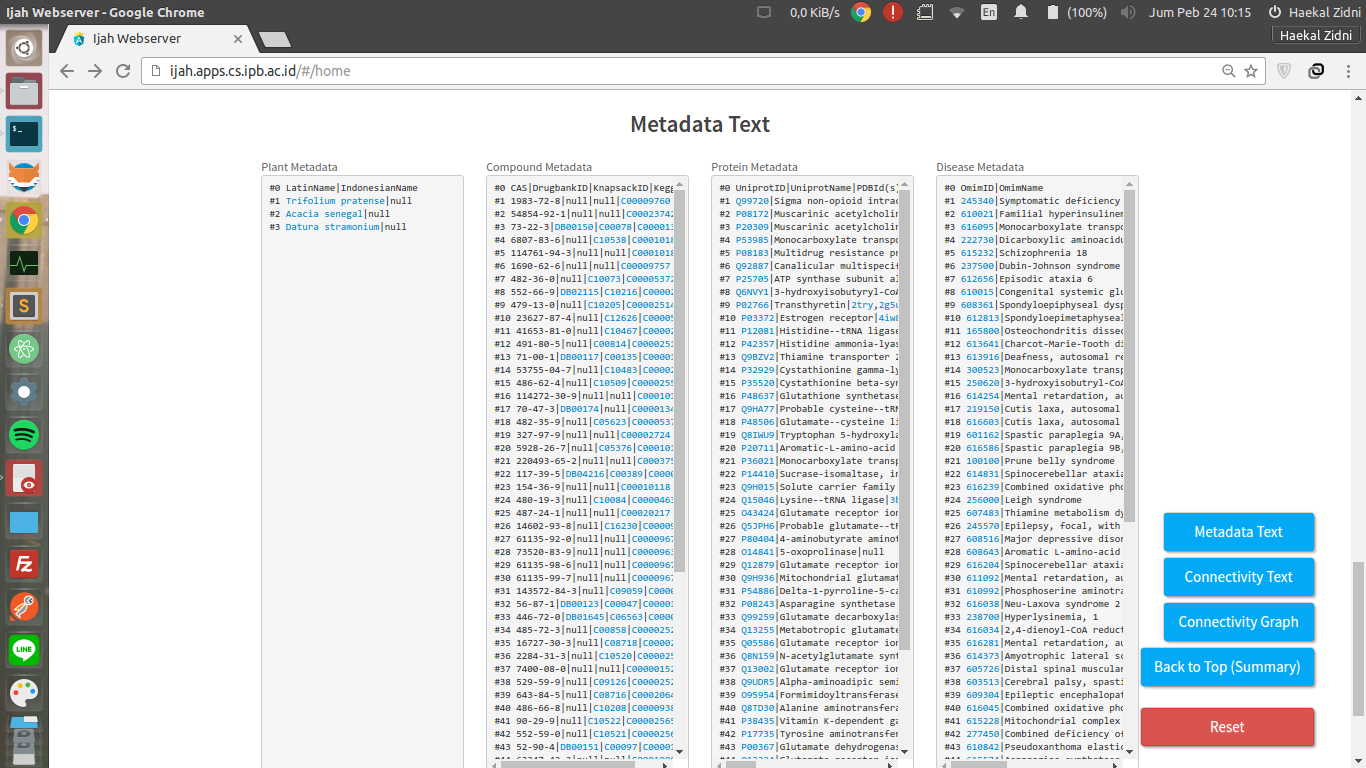
\includegraphics[scale=0.3]{ijah_example_2a_meta.png}
	\caption{Metadata Text Output pada use case Plant Search Only}
	\label{fig:ijah_example_2a_meta}
\end{figure}

\section{Compound Search Only}
Contoh lain dari \emph{use case} Drug-Side Only yaitu Compound Search Only dimana perbedaannya hanya pada input, yaitu menginputkan senyawa (Compound) untuk mencari semua (Plant, Protein, Disease) yang terkait dengan senyawa yang diinputkan.

